\PassOptionsToPackage{unicode}{hyperref}
\PassOptionsToPackage{hyphens}{url}

\documentclass[UTF-8]{ctexart}
\usepackage{geometry}
\geometry{margin=1.5cm, vmargin={0pt,1cm}}
\setlength{\topmargin}{-1cm}
\setlength{\paperheight}{29.7cm}
\setlength{\textheight}{25.3cm}

% useful packages.
\usepackage{amsfonts}
\usepackage{amsmath}
\usepackage{amssymb}
\usepackage{amsthm}
\usepackage{enumerate}
\usepackage{graphicx}
\usepackage{multicol}
\usepackage{fancyhdr}
\usepackage{layout}
\usepackage{subfigure}
\usepackage{float}
\usepackage{color}
\usepackage{url}
\usepackage{listings}
\usepackage[framed,numbered,autolinebreaks,useliterate]{mcode} 
\usepackage{multicol} 
\usepackage{lmodern}
\usepackage{amssymb,amsmath}
\usepackage{ifxetex,ifluatex}
\ifnum 0\ifxetex 1\fi\ifluatex 1\fi=0 % if pdftex
\usepackage[T1]{fontenc}
\usepackage[utf8]{inputenc}
\usepackage{textcomp} % provide euro and other symbols
\else % if luatex or xetex
\usepackage{unicode-math}
\defaultfontfeatures{Scale=MatchLowercase}
\defaultfontfeatures[\rmfamily]{Ligatures=TeX,Scale=1}
\fi
% Use upquote if available, for straight quotes in verbatim environments
\IfFileExists{upquote.sty}{\usepackage{upquote}}{}
\IfFileExists{microtype.sty}{% use microtype if available
	\usepackage[]{microtype}
	\UseMicrotypeSet[protrusion]{basicmath} % disable protrusion for tt fonts
}{}
\makeatletter
\@ifundefined{KOMAClassName}{% if non-KOMA class
	\IfFileExists{parskip.sty}{%
		\usepackage{parskip}
	}{% else
		\setlength{\parindent}{0pt}
		\setlength{\parskip}{6pt plus 2pt minus 1pt}}
}{% if KOMA class
	\KOMAoptions{parskip=half}}
\makeatother
\usepackage{xcolor}
\IfFileExists{xurl.sty}{\usepackage{xurl}}{} % add URL line breaks if available
\IfFileExists{bookmark.sty}{\usepackage{bookmark}}{\usepackage{hyperref}}
\hypersetup{
	pdftitle={BostonHousePrice},
	pdfauthor={沈鼎涛},
	hidelinks,
	pdfcreator={LaTeX via pandoc}}
\urlstyle{same} % disable monospaced font for URLs
\usepackage{fancyvrb}
\newcommand{\VerbBar}{|}
\newcommand{\VERB}{\Verb[commandchars=\\\{\}]}
\DefineVerbatimEnvironment{Highlighting}{Verbatim}{commandchars=\\\{\}}
% Add ',fontsize=\small' for more characters per line
\usepackage{framed}
\definecolor{shadecolor}{RGB}{248,248,248}
\newenvironment{Shaded}{\begin{snugshade}}{\end{snugshade}}
\newcommand{\AlertTok}[1]{\textcolor[rgb]{0.94,0.16,0.16}{#1}}
\newcommand{\AnnotationTok}[1]{\textcolor[rgb]{0.56,0.35,0.01}{\textbf{\textit{#1}}}}
\newcommand{\AttributeTok}[1]{\textcolor[rgb]{0.77,0.63,0.00}{#1}}
\newcommand{\BaseNTok}[1]{\textcolor[rgb]{0.00,0.00,0.81}{#1}}
\newcommand{\BuiltInTok}[1]{#1}
\newcommand{\CharTok}[1]{\textcolor[rgb]{0.31,0.60,0.02}{#1}}
\newcommand{\CommentTok}[1]{\textcolor[rgb]{0.56,0.35,0.01}{\textit{#1}}}
\newcommand{\CommentVarTok}[1]{\textcolor[rgb]{0.56,0.35,0.01}{\textbf{\textit{#1}}}}
\newcommand{\ConstantTok}[1]{\textcolor[rgb]{0.00,0.00,0.00}{#1}}
\newcommand{\ControlFlowTok}[1]{\textcolor[rgb]{0.13,0.29,0.53}{\textbf{#1}}}
\newcommand{\DataTypeTok}[1]{\textcolor[rgb]{0.13,0.29,0.53}{#1}}
\newcommand{\DecValTok}[1]{\textcolor[rgb]{0.00,0.00,0.81}{#1}}
\newcommand{\DocumentationTok}[1]{\textcolor[rgb]{0.56,0.35,0.01}{\textbf{\textit{#1}}}}
\newcommand{\ErrorTok}[1]{\textcolor[rgb]{0.64,0.00,0.00}{\textbf{#1}}}
\newcommand{\ExtensionTok}[1]{#1}
\newcommand{\FloatTok}[1]{\textcolor[rgb]{0.00,0.00,0.81}{#1}}
\newcommand{\FunctionTok}[1]{\textcolor[rgb]{0.00,0.00,0.00}{#1}}
\newcommand{\ImportTok}[1]{#1}
\newcommand{\InformationTok}[1]{\textcolor[rgb]{0.56,0.35,0.01}{\textbf{\textit{#1}}}}
\newcommand{\KeywordTok}[1]{\textcolor[rgb]{0.13,0.29,0.53}{\textbf{#1}}}
\newcommand{\NormalTok}[1]{#1}
\newcommand{\OperatorTok}[1]{\textcolor[rgb]{0.81,0.36,0.00}{\textbf{#1}}}
\newcommand{\OtherTok}[1]{\textcolor[rgb]{0.56,0.35,0.01}{#1}}
\newcommand{\PreprocessorTok}[1]{\textcolor[rgb]{0.56,0.35,0.01}{\textit{#1}}}
\newcommand{\RegionMarkerTok}[1]{#1}
\newcommand{\SpecialCharTok}[1]{\textcolor[rgb]{0.00,0.00,0.00}{#1}}
\newcommand{\SpecialStringTok}[1]{\textcolor[rgb]{0.31,0.60,0.02}{#1}}
\newcommand{\StringTok}[1]{\textcolor[rgb]{0.31,0.60,0.02}{#1}}
\newcommand{\VariableTok}[1]{\textcolor[rgb]{0.00,0.00,0.00}{#1}}
\newcommand{\VerbatimStringTok}[1]{\textcolor[rgb]{0.31,0.60,0.02}{#1}}
\newcommand{\WarningTok}[1]{\textcolor[rgb]{0.56,0.35,0.01}{\textbf{\textit{#1}}}}
\usepackage{graphicx,grffile}
\makeatletter
\def\maxwidth{\ifdim\Gin@nat@width>\linewidth\linewidth\else\Gin@nat@width\fi}
\def\maxheight{\ifdim\Gin@nat@height>\textheight\textheight\else\Gin@nat@height\fi}
\makeatother
% Scale images if necessary, so that they will not overflow the page
% margins by default, and it is still possible to overwrite the defaults
% using explicit options in \includegraphics[width, height, ...]{}
\setkeys{Gin}{width=\maxwidth,height=\maxheight,keepaspectratio}
% Set default figure placement to htbp
\makeatletter
\def\fps@figure{htbp}
\makeatother
\setlength{\emergencystretch}{3em} % prevent overfull lines
\providecommand{\tightlist}{%
	\setlength{\itemsep}{0pt}\setlength{\parskip}{0pt}}
\setcounter{secnumdepth}{-\maxdimen} % remove section numbering

% some common command
\newcommand{\dif}{\mathrm{d}}
\newcommand{\avg}[1]{\left\langle #1 \right\rangle}
\newcommand{\difFrac}[2]{\frac{\dif #1}{\dif #2}}
\newcommand{\pdfFrac}[2]{\frac{\partial #1}{\partial #2}}
\newcommand{\OFL}{\mathrm{OFL}}
\newcommand{\UFL}{\mathrm{UFL}}
\newcommand{\fl}{\mathrm{fl}}
\newcommand{\op}{\odot}
\newcommand{\Eabs}{E_{\mathrm{abs}}}
\newcommand{\Erel}{E_{\mathrm{rel}}}

\begin{document}
	
	\pagestyle{fancy}
	\fancyhead{}
	\lhead{2020}
	\chead{数学实践大作业}
	\rhead{沈鼎涛3170104764}
	
	\begin{center}
	\begin{LARGE}
		波士顿郊区房价数据集可视化分析 \\
		与房价预测模型的构建{\tiny }
	\end{LARGE}
	\vspace{0.5cm}
	
	\begin{Large}
		沈鼎涛 3170104764
	\end{Large}
	\end{center}
	\vspace{0.5cm}
	
	\tableofcontents
	
	\newpage
	
	\section{1 背景}
	
	\subsection{1.1 问题介绍}
	我们针对MASS包中内置的波士顿郊区的房价数据集(Housing Values in Suburbs of Boston),进行数据的分析和可视化呈现,并根据数据集构造波士顿郊区的房价预测模型。基于此,我们着眼的具体问题是:
	\begin{itemize}
		\item 分析波士顿郊区各社会指标与房价的相关关系;
		\item 分析波士顿郊区房价分布概况、主要影响因素及其作用;
		\item 构建房屋报价的预测模型,并用数据进行参数拟合;
		\item 对模型进行统计检验和真实数据测试等。
	\end{itemize}
	\subsection{1.2 数据集介绍}
	波士顿房价数据集是统计的20世纪70年代中期波士顿郊区房价的中位数,统计了包括自有住房报价中位数的当时郊区部分犯罪率、房产税等13个指标,数据量相应指标的详细信息如下:
	\begin{center}
		\begin{tabular}{|c|c|} 
			\hline 
			\multicolumn{2}{|c|}{Boston{MASS}:Housing Values in Suburbs of Boston} \\ 
			\hline 
			crim&城镇人均犯罪率\\
			zn &占地面积超过25,000平方英尺的住宅用地比例\\
			indus &每个城镇非零售业务的比例\\
			chas & Charles River虚拟变量(如果是河道,则为1;否则为0)\\
			nox & 一氧化氮浓度(每千万份)\\
			rm & 每间住宅的平均房间数 \\
			age & 1940年以前建造的自住单位比例 \\
			dis & 到波士顿的五个就业中心的加权距离 \\
			rad & 径向高速公路的可达性指数 \\
			tax & 每10,000美元的全额财产税税率 \\
			ptratio & 城镇的学生与教师比例 \\
			black & $1000(Bk- 0.63)^{2}$其中Bk是城镇黑人的比例 \\
			lstat & 低阶层人口百分比 \\
			medv & 自有住房的报价中位数(单位1000美元) \\
			\hline 
		\end{tabular}
	\end{center}

	数据集共包括506个案例的记录,数据规模较小,但作为经典案例数据集,常用于数据可视化、回归分析以及机器学习等。

	\subsection{1.3 知识背景和技术工具}
	\begin{itemize}
		\item 理论知识 \begin{itemize}
			\item R语言基础;基于tidyverse的数据处理;基于ggplot2的数据可视化等。
			\item 统计知识:线性回归、非线性回归、统计检验等。
		\end{itemize}
		\item 技术工具和平台 \begin{itemize}
			\item RStudio
		\end{itemize}
	\end{itemize}
	
	\section{2 数据处理}
	
	\subsection{2.1 数据集加载}
	数据集的载入
	
\begin{Shaded}
\begin{Highlighting}[]
\KeywordTok{library}\NormalTok{(MASS)}
\KeywordTok{attach}\NormalTok{(Boston)}
\end{Highlighting}
\end{Shaded}
	
	查看Boston数据集的维数和结构:
	
	\begin{Shaded}
	\begin{Highlighting}[]
\KeywordTok{glimpse}\NormalTok{(Boston)}
	\end{Highlighting}
	\end{Shaded}
	
	\begin{verbatim}
	## Rows: 506
	## Columns: 14
	## $ crim    <dbl> 0.00632, 0.02731, 0.02729, 0.03237, 0.06905, 0.02985, 0.088...
	## $ zn      <dbl> 18.0, 0.0, 0.0, 0.0, 0.0, 0.0, 12.5, 12.5, 12.5, 12.5, 12.5...
	## $ indus   <dbl> 2.31, 7.07, 7.07, 2.18, 2.18, 2.18, 7.87, 7.87, 7.87, 7.87,...
	## $ chas    <int> 0, 0, 0, 0, 0, 0, 0, 0, 0, 0, 0, 0, 0, 0, 0, 0, 0, 0, 0, 0,...
	## $ nox     <dbl> 0.538, 0.469, 0.469, 0.458, 0.458, 0.458, 0.524, 0.524, 0.5...
	## $ rm      <dbl> 6.575, 6.421, 7.185, 6.998, 7.147, 6.430, 6.012, 6.172, 5.6...
	## $ age     <dbl> 65.2, 78.9, 61.1, 45.8, 54.2, 58.7, 66.6, 96.1, 100.0, 85.9...
	## $ dis     <dbl> 4.0900, 4.9671, 4.9671, 6.0622, 6.0622, 6.0622, 5.5605, 5.9...
	## $ rad     <int> 1, 2, 2, 3, 3, 3, 5, 5, 5, 5, 5, 5, 5, 4, 4, 4, 4, 4, 4, 4,...
	## $ tax     <dbl> 296, 242, 242, 222, 222, 222, 311, 311, 311, 311, 311, 311,...
	## $ ptratio <dbl> 15.3, 17.8, 17.8, 18.7, 18.7, 18.7, 15.2, 15.2, 15.2, 15.2,...
	## $ black   <dbl> 396.90, 396.90, 392.83, 394.63, 396.90, 394.12, 395.60, 396...
	## $ lstat   <dbl> 4.98, 9.14, 4.03, 2.94, 5.33, 5.21, 12.43, 19.15, 29.93, 17...
	## $ medv    <dbl> 24.0, 21.6, 34.7, 33.4, 36.2, 28.7, 22.9, 27.1, 16.5, 18.9,...
	\end{verbatim}
	
	查看Boston数据集的基本统计量
	
	\begin{Shaded}
	\begin{Highlighting}[]
\KeywordTok{summary}\NormalTok{(Boston)}
	\end{Highlighting}
	\end{Shaded}
	
	\begin{verbatim}
	##       crim                zn             indus            chas        
	##  Min.   : 0.00632   Min.   :  0.00   Min.   : 0.46   Min.   :0.00000  
	##  1st Qu.: 0.08205   1st Qu.:  0.00   1st Qu.: 5.19   1st Qu.:0.00000  
	##  Median : 0.25651   Median :  0.00   Median : 9.69   Median :0.00000  
	##  Mean   : 3.61352   Mean   : 11.36   Mean   :11.14   Mean   :0.06917  
	##  3rd Qu.: 3.67708   3rd Qu.: 12.50   3rd Qu.:18.10   3rd Qu.:0.00000  
	##  Max.   :88.97620   Max.   :100.00   Max.   :27.74   Max.   :1.00000  
	##       nox               rm             age              dis        
	##  Min.   :0.3850   Min.   :3.561   Min.   :  2.90   Min.   : 1.130  
	##  1st Qu.:0.4490   1st Qu.:5.886   1st Qu.: 45.02   1st Qu.: 2.100  
	##  Median :0.5380   Median :6.208   Median : 77.50   Median : 3.207  
	##  Mean   :0.5547   Mean   :6.285   Mean   : 68.57   Mean   : 3.795  
	##  3rd Qu.:0.6240   3rd Qu.:6.623   3rd Qu.: 94.08   3rd Qu.: 5.188  
	##  Max.   :0.8710   Max.   :8.780   Max.   :100.00   Max.   :12.127  
	##       rad              tax           ptratio          black       
	##  Min.   : 1.000   Min.   :187.0   Min.   :12.60   Min.   :  0.32  
	##  1st Qu.: 4.000   1st Qu.:279.0   1st Qu.:17.40   1st Qu.:375.38  
	##  Median : 5.000   Median :330.0   Median :19.05   Median :391.44  
	##  Mean   : 9.549   Mean   :408.2   Mean   :18.46   Mean   :356.67  
	##  3rd Qu.:24.000   3rd Qu.:666.0   3rd Qu.:20.20   3rd Qu.:396.23  
	##  Max.   :24.000   Max.   :711.0   Max.   :22.00   Max.   :396.90  
	##      lstat            medv      
	##  Min.   : 1.73   Min.   : 5.00  
	##  1st Qu.: 6.95   1st Qu.:17.02  
	##  Median :11.36   Median :21.20  
	##  Mean   :12.65   Mean   :22.53  
	##  3rd Qu.:16.95   3rd Qu.:25.00  
	##  Max.   :37.97   Max.   :50.00
	\end{verbatim}
	
	\subsection{2.2 数据预处理}
	检查Boston数据集是否包含缺失值或重复值:
	
	\begin{Shaded}
		\begin{Highlighting}[]
\KeywordTok{any}\NormalTok{(}\KeywordTok{is.na}\NormalTok{(Boston))}
		\end{Highlighting}
	\end{Shaded}
	
	\begin{verbatim}
	## [1] FALSE
	\end{verbatim}
	
\begin{Shaded}
\begin{Highlighting}[]
\KeywordTok{any}\NormalTok{(}\KeywordTok{duplicated}\NormalTok{(Boston))}
\end{Highlighting}
\end{Shaded}
	
	\begin{verbatim}
	## [1] FALSE
	\end{verbatim}
	
	结果均为\texttt{FALSE},说明Boston数据集无缺失值或重复值,不需要进行数据清洗。
	
	\section{3 数据可视化与分析}
	\subsection{3.1 相关性分析}
	Boston数据集中包含14个变量,首先计算其两两之间的相关系数,得到相关系数矩阵\texttt{coor\_matrix},并对其进行可视化处理:
	
	\begin{Shaded}
		\begin{Highlighting}[]
\NormalTok{corr_matrix<-}\KeywordTok{cor}\NormalTok{(Boston)}
\KeywordTok{corrplot}\NormalTok{(corr_matrix,}\DataTypeTok{method=}\StringTok{"number"}\NormalTok{, }\DataTypeTok{type=}\StringTok{"upper"}\NormalTok{,}\DataTypeTok{diag=}\OtherTok{FALSE}\NormalTok{)}
		\end{Highlighting}
	\end{Shaded}

\begin{figure}[H]
	\centering
	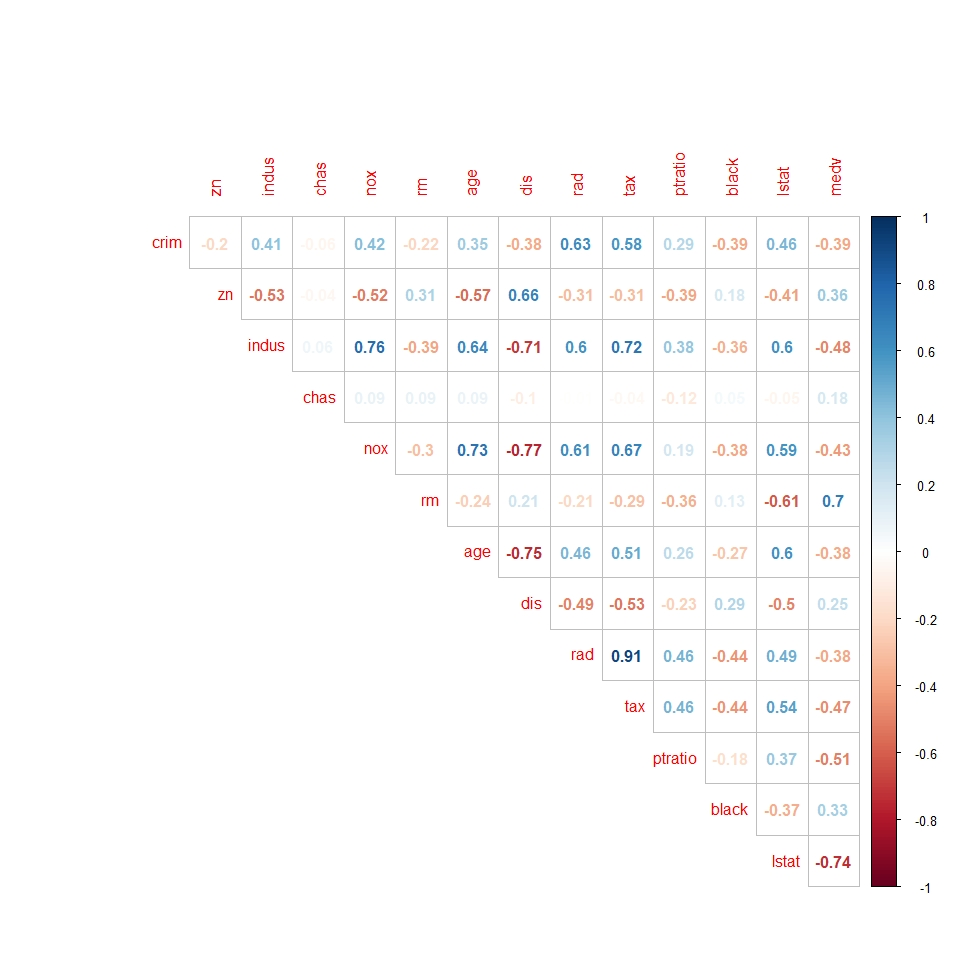
\includegraphics[width=0.9\linewidth]{cormatrix}
	%\caption{基于Wolfe条件的线搜索算法}
	\label{bdc1}
\end{figure}

由上述相关系数矩阵我们可以得出一些结论:

\begin{itemize}
	\item rad与tax有0.91的强正相关关系,这意味着随着径向公路可达性的增加,每10,000美元的全价房产税率也随之增加
	\item crim与变量rad和tax密切相关,这意味着径向公路的可达性增加,人均犯罪率增加.
	\item nox与indus有很强的正相关性,与dis有较强的负相关性,而这支持了工业地区氮氧化物浓度高的观点.
	\item dis和age具有较强的负相关性,距离就业中心越近的房屋年代普遍更新.
	\item medv和rm具有较强的正相关性,与lstat具有较强的负相关性等.
\end{itemize}

\subsection{3.2 房屋报价中位数(medv)分析}

在上述所有指标相互间的相关关系中,我们最为关心房价中值(medv)和其余变量的相关关系,做medv同其他13个指标的散点图:

\begin{Shaded}
	\begin{Highlighting}[]
		\NormalTok{Boston }\OperatorTok
			\StringTok{  }\KeywordTok{gather}\NormalTok{(var, val, }\OperatorTok{-}\NormalTok{medv) }\OperatorTok
				\StringTok{  }\KeywordTok{ggplot}\NormalTok{(}\KeywordTok{aes}\NormalTok{(}\DataTypeTok{x =}\NormalTok{ val, }\DataTypeTok{y =}\NormalTok{ medv)) }\OperatorTok{+}
				\StringTok{  }\KeywordTok{geom_point}\NormalTok{() }\OperatorTok{+}
				\StringTok{  }\KeywordTok{geom_smooth}\NormalTok{(}\DataTypeTok{method =} \StringTok{"lm"}\NormalTok{, }\DataTypeTok{se =} \OtherTok{TRUE}\NormalTok{, }\DataTypeTok{col =} \StringTok{"blue"}\NormalTok{) }\OperatorTok{+}
				\StringTok{  }\KeywordTok{facet_wrap}\NormalTok{(}\OperatorTok{~}\NormalTok{var, }\DataTypeTok{scales =} \StringTok{"free"}\NormalTok{) }\OperatorTok{+}
				\StringTok{  }\KeywordTok{theme_gray}\NormalTok{() }\OperatorTok{+}
				\StringTok{  }\KeywordTok{ggtitle}\NormalTok{(}\StringTok{"房价中值与其他变量的散点图及拟合"}\NormalTok{) }
			\end{Highlighting}
		\end{Shaded}	
		\begin{figure}[H]
			\centering
			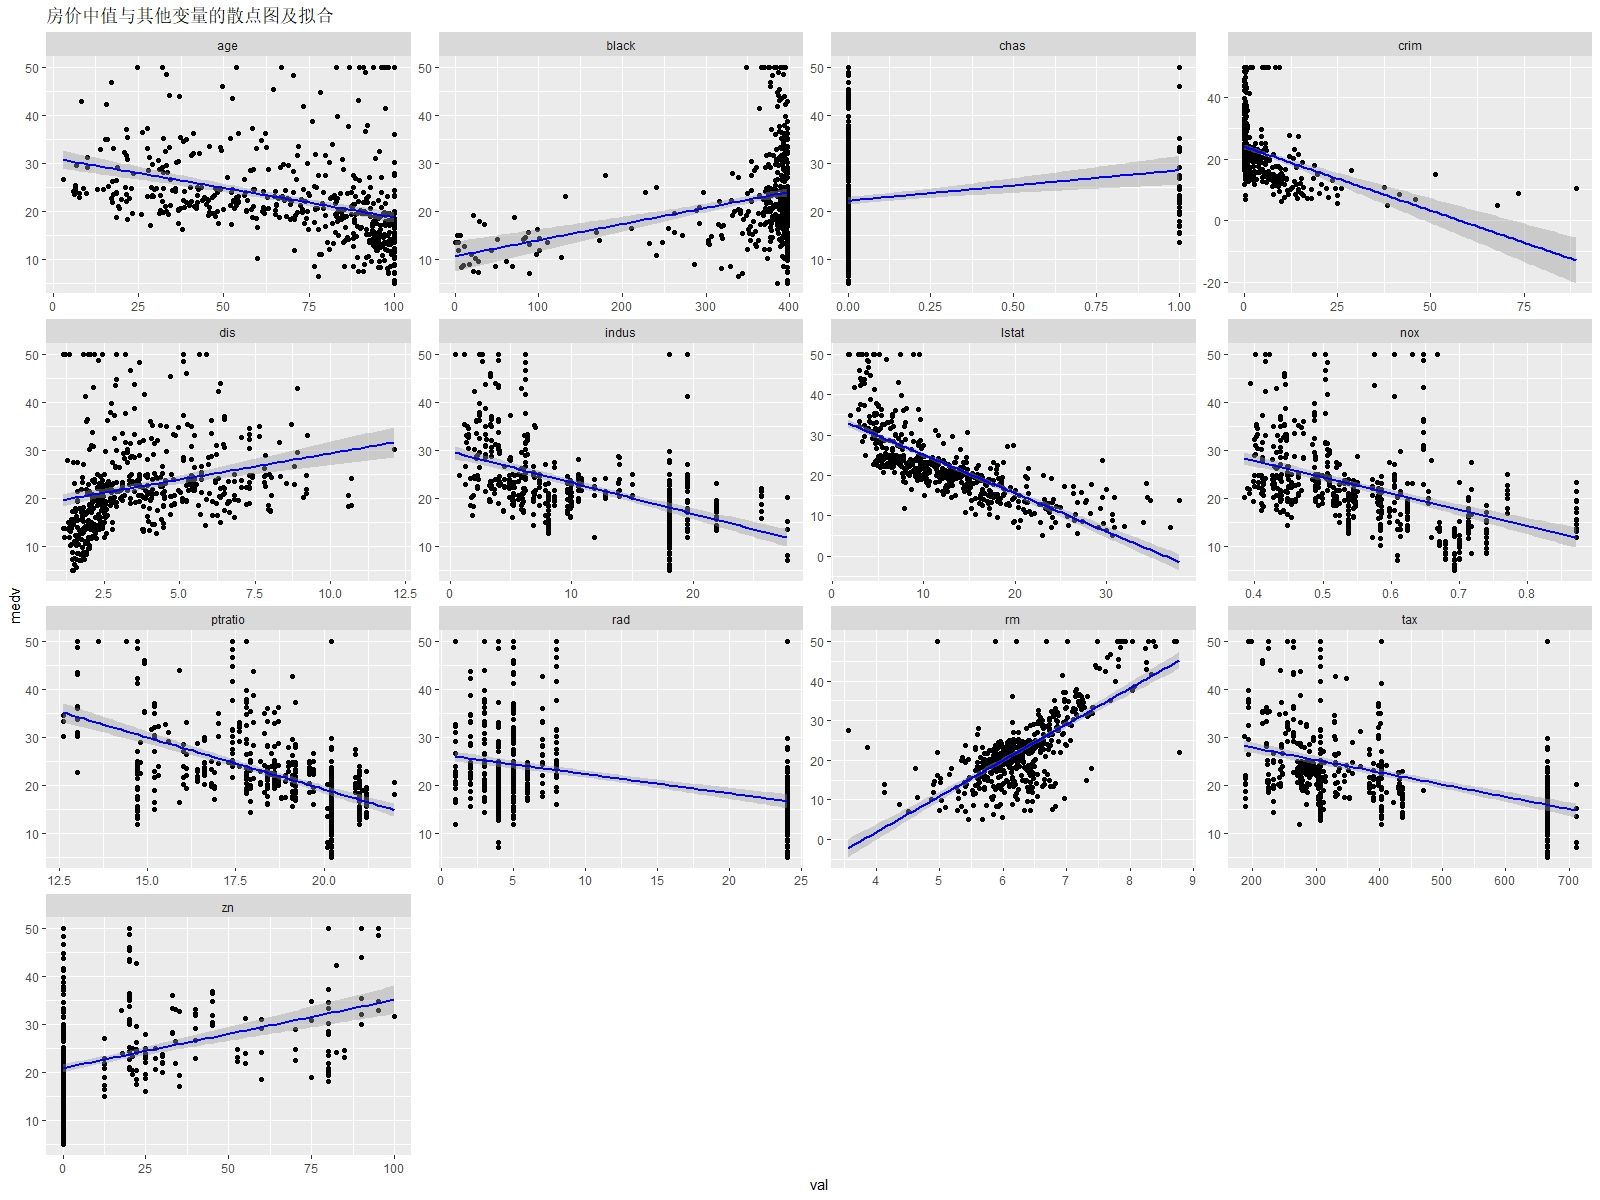
\includegraphics[width=0.9\linewidth]{medv_val}
			%\caption{基于Wolfe条件的线搜索算法}
			\label{bdc1}
		\end{figure}	
		
		
可以明显地看到,房价中值(medv)和平均房间数(rm)具有较为显著的正相关关系,和低收入人口比例(lstat)具有较为显著的负相关关系。rm属于房屋自身性质,而lstat属于地区的社会属性,我们对后者对medv的影响更感兴趣。

首先根据虚拟变量chas,即是否临近Charles河,做出medv分布的直方图:

\begin{Shaded}
	\begin{Highlighting}[]
\NormalTok{Boston}\OperatorTok{$}\NormalTok{chas=}\KeywordTok{factor}\NormalTok{(Boston}\OperatorTok{$}\NormalTok{chas)}
\KeywordTok{ggplot}\NormalTok{(Boston, }\KeywordTok{aes}\NormalTok{(}\DataTypeTok{x =}\NormalTok{ medv, }\DataTypeTok{fill =}\NormalTok{ chas)) }\OperatorTok{+}
\StringTok{  }\KeywordTok{geom_histogram}\NormalTok{(}\DataTypeTok{position =} \StringTok{"identity"}\NormalTok{, }\DataTypeTok{alpha =} \FloatTok{0.4}\NormalTok{,}\DataTypeTok{bins=}\DecValTok{30}\NormalTok{)}\OperatorTok{+}
\StringTok{  }\KeywordTok{ggtitle}\NormalTok{(}\StringTok{"房价中值(medv)的频数分布直方图(按是否临近查尔斯河分类)"}\NormalTok{)}
	\end{Highlighting}
\end{Shaded}
	\begin{figure}[H]
		\centering
		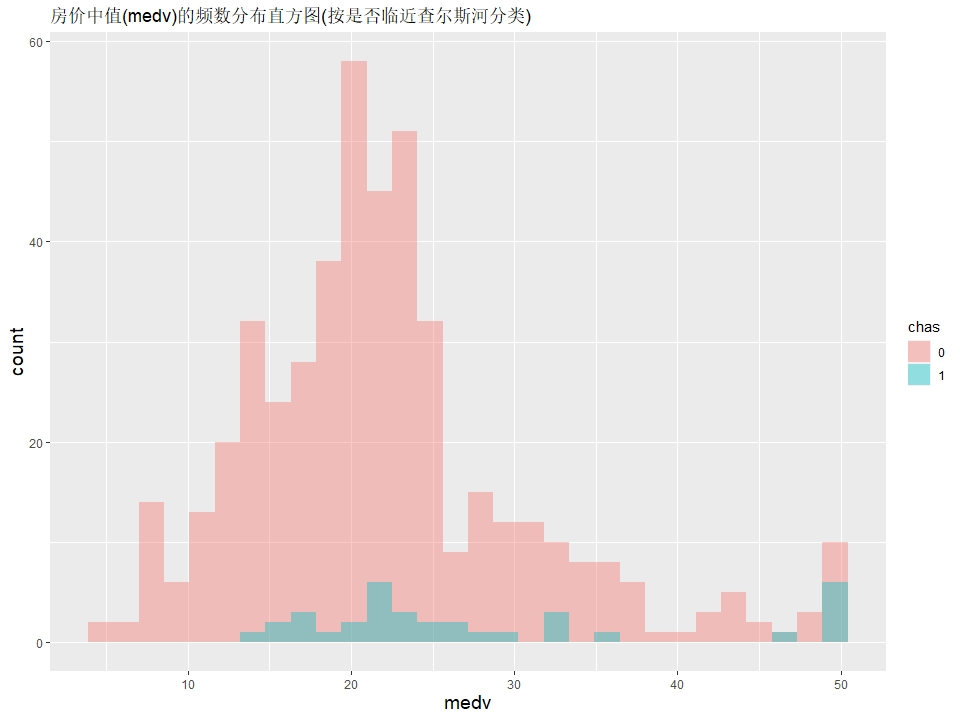
\includegraphics[width=0.7\linewidth]{zhifangtu3}
		%\caption{基于Wolfe条件的线搜索算法}
		\label{bdc1}
	\end{figure}

查看medv的相关统计量为:

\begin{Shaded}
	\begin{Highlighting}[]
\KeywordTok{summary}\NormalTok{(Boston}\OperatorTok{$}\NormalTok{medv)}
	\end{Highlighting}
\end{Shaded}
		
\begin{verbatim}
##    Min. 1st Qu.  Median    Mean 3rd Qu.    Max. 
##    5.00   17.02   21.20   22.53   25.00   50.00
\end{verbatim}

然后做lstat分布的直方图

\begin{Shaded}
	\begin{Highlighting}[]
\KeywordTok{ggplot}\NormalTok{(Boston, }\KeywordTok{aes}\NormalTok{(}\DataTypeTok{x =}\NormalTok{ lstat)) }\OperatorTok{+}
\StringTok{  }\KeywordTok{geom_histogram}\NormalTok{(}\DataTypeTok{position =} \StringTok{"identity"}\NormalTok{, }\DataTypeTok{alpha =} \FloatTok{0.4}\NormalTok{,}\DataTypeTok{bins=}\DecValTok{30}\NormalTok{,}\DataTypeTok{fill=}\StringTok{"orange"}\NormalTok{)}\OperatorTok{+}
\StringTok{  }\KeywordTok{ggtitle}\NormalTok{(}\StringTok{"低阶层人口比例(lstat)的频数分布直方图"}\NormalTok{)}\OperatorTok{+}
\StringTok{  }\KeywordTok{theme}\NormalTok{(}\DataTypeTok{axis.title.x =}\KeywordTok{element_text}\NormalTok{(}\DataTypeTok{size=}\DecValTok{14}\NormalTok{),}
\DataTypeTok{axis.title.y=}\KeywordTok{element_text}\NormalTok{(}\DataTypeTok{size=}\DecValTok{14}\NormalTok{))}
	\end{Highlighting}
\end{Shaded}

\begin{figure}[H]
	\centering
	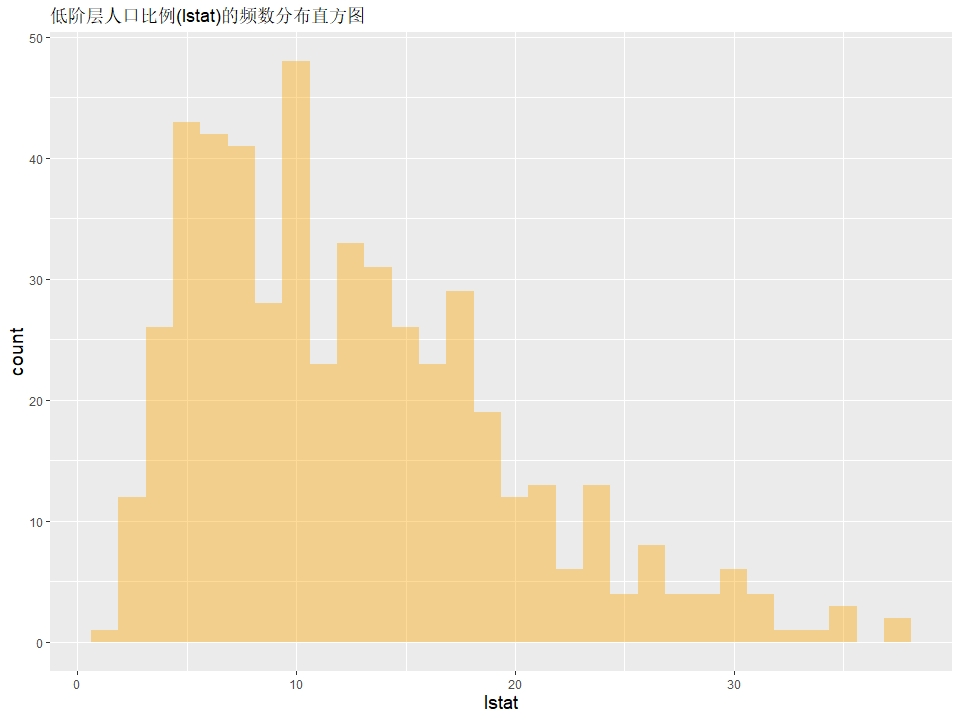
\includegraphics[width=0.7\linewidth]{histo2}
	%\caption{基于Wolfe条件的线搜索算法}
	\label{bdc1}
\end{figure}
查看lstat统计量:

\begin{Shaded}
	\begin{Highlighting}[]
\KeywordTok{summary}\NormalTok{(Boston}\OperatorTok{$}\NormalTok{lstat)}
		\end{Highlighting}
\end{Shaded}
		
\begin{verbatim}
##    Min. 1st Qu.  Median    Mean 3rd Qu.    Max. 
##    1.73    6.95   11.36   12.65   16.95   37.97
\end{verbatim}
		
给Boston数据集添加一个统计量lstat\_lev,表示低阶级人口比例水平,根据lstat的数据(median=11.36\%)我们定义:当lstat\textless=11.36,lstat\_lev=0,表征低阶级群体比例较低;lstat\textgreater11.36,lstat\_lev=1,表征低阶级人口群体比例较高.
		
		\begin{Shaded}
			\begin{Highlighting}[]
\NormalTok{Boston1<-Boston }\OperatorTok\StringTok{ }
	\StringTok{  }\KeywordTok{mutate}\NormalTok{(}\DataTypeTok{lstat_lev =} \KeywordTok{ifelse}\NormalTok{(lstat}\OperatorTok{>}\FloatTok{11.36}\NormalTok{, }\DecValTok{1}\NormalTok{, }\DecValTok{0}\NormalTok{))}
				\end{Highlighting}
			\end{Shaded}
			
根据lstat\_lev分类,绘制medv的箱线图:
			
\begin{Shaded}
	\begin{Highlighting}[]
\NormalTok{Boston1}\OperatorTok{$}\NormalTok{lstat_lev=}\KeywordTok{factor}\NormalTok{(Boston1}\OperatorTok{$}\NormalTok{lstat_lev)}
\KeywordTok{ggplot}\NormalTok{(Boston1, }\KeywordTok{aes}\NormalTok{(}\DataTypeTok{y =}\NormalTok{ medv, }\DataTypeTok{fill =}\NormalTok{ lstat_lev)) }\OperatorTok{+}
\StringTok{  }\KeywordTok{geom_boxplot}\NormalTok{()}\OperatorTok{+}
\StringTok{  }\KeywordTok{ggtitle}\NormalTok{(}\StringTok{"房价中值(medv)箱线图(按lstat水平)"}\NormalTok{)}\OperatorTok{+}
\StringTok{  }\KeywordTok{theme}\NormalTok{(}\DataTypeTok{axis.title.x =}\KeywordTok{element_text}\NormalTok{(}\DataTypeTok{size=}\DecValTok{14}\NormalTok{),}
\DataTypeTok{axis.title.y=}\KeywordTok{element_text}\NormalTok{(}\DataTypeTok{size=}\DecValTok{14}\NormalTok{))}
				\end{Highlighting}
			\end{Shaded}

\begin{figure}[H]
	\centering
	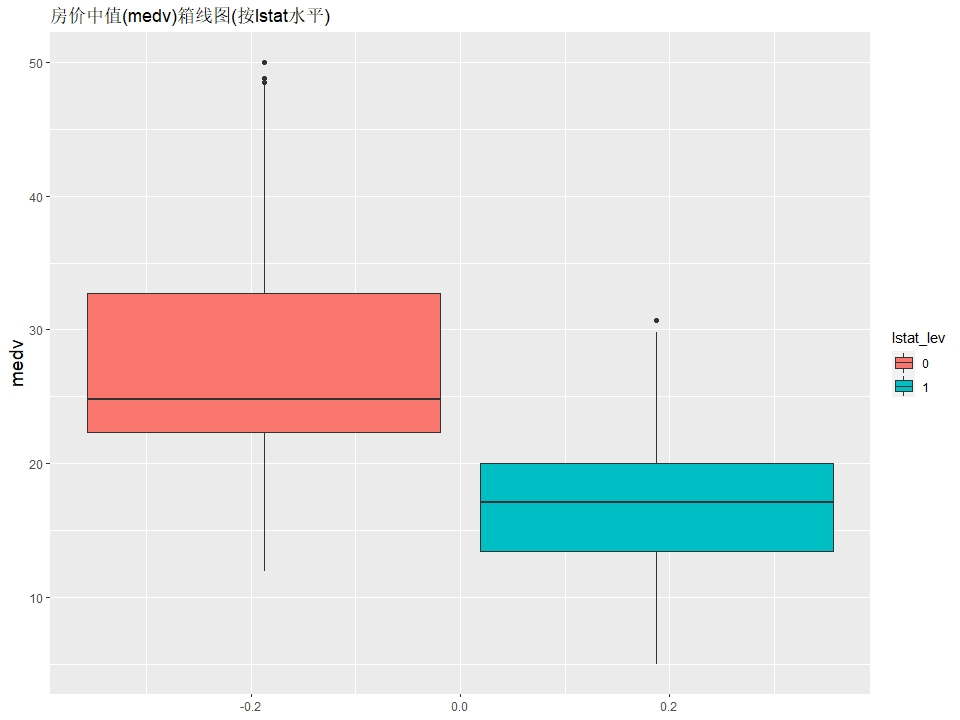
\includegraphics[width=0.7\linewidth]{box}
	%\caption{基于Wolfe条件的线搜索算法}
	\label{bdc1}
\end{figure}

由箱线图可以看出,lstat水平不同的地区,medv的差异十分明显,低阶层人口比例较高的地区的整体medv水平更高。由此也印证了lstat和medv之间较为显著的相关关系。

\section{4 房屋报价中值(medv)预测模型}

首先,将数据按3:1划分为训练集Boston.train和测试集Boston.test
\begin{Shaded}
	\begin{Highlighting}[]
\KeywordTok{data}\NormalTok{(Boston)}
\NormalTok{smp_size<-}\KeywordTok{floor}\NormalTok{(}\FloatTok{0.75}\OperatorTok{*}\KeywordTok{nrow}\NormalTok{(Boston))}
\KeywordTok{set.seed}\NormalTok{(}\DecValTok{12}\NormalTok{)}
\NormalTok{train_index<-}\KeywordTok{sample}\NormalTok{(}\KeywordTok{seq_len}\NormalTok{(}\KeywordTok{nrow}\NormalTok{(Boston)), }\DataTypeTok{size=}\NormalTok{smp_size)}
\NormalTok{Boston.train<-Boston[train_index, ]}
\NormalTok{Boston.test<-Boston[}\OperatorTok{-}\NormalTok{train_index, ]}
	\end{Highlighting}
\end{Shaded}

我们利用训练集的数据进行参数拟合,并在测试集上测试模型的拟合效果。对于模型的选取,我们尝试以下几种模型构造:
\begin{itemize}
	\item 简单的单变量线性回归模型
	\item 单变量非线性回归模型
	\item 多变量回归模型
\end{itemize}

\subsection{4.1 简单的单变量线性回归模型}
对于模型变量的选择,根据上一节的相关性分析,低收入人口比例lstat与medv的相关性最为显著,因此我们优先选择该变量来构造简单单变量线性回归模型。
\begin{Shaded}
	\begin{Highlighting}[]
\NormalTok{model.slm=}\KeywordTok{lm}\NormalTok{(medv}\OperatorTok{~}\NormalTok{lstat,}\DataTypeTok{data=}\NormalTok{Boston.train)}
	\end{Highlighting}
\end{Shaded}

查看其统计量:

\begin{Shaded}
	\begin{Highlighting}[]
\KeywordTok{summary}\NormalTok{(model.slm)}
	\end{Highlighting}
\end{Shaded}

\begin{verbatim}
## 
## Call:
## lm(formula = medv ~ lstat, data = Boston.train)
## 
## Residuals:
##     Min      1Q  Median      3Q     Max 
## -14.800  -3.753  -1.161   1.690  24.242 
## 
## Coefficients:
##             Estimate Std. Error t value Pr(>|t|)    
## (Intercept) 34.12056    0.63739   53.53   <2e-16 ***
## lstat       -0.94171    0.04372  -21.54   <2e-16 ***
## ---
## Signif. codes:  0 '***' 0.001 '**' 0.01 '*' 0.05 '.' 0.1 ' ' 1
## 
## Residual standard error: 6.007 on 377 degrees of freedom
## Multiple R-squared:  0.5517, Adjusted R-squared:  0.5505 
## F-statistic:   464 on 1 and 377 DF,  p-value: < 2.2e-16
\end{verbatim}

通过查看模型的结果数据,我们可以发现通过T检验的截距和自变量lstat都是非常显著。我们首先在测试集上进行预测和误差分析:

\begin{Shaded}
	\begin{Highlighting}[]
\KeywordTok{library}\NormalTok{(Metrics)}
\NormalTok{model1.evaluate<-}\KeywordTok{predict}\NormalTok{(model.slm, Boston.test) }
\KeywordTok{ggplot}\NormalTok{(}\DataTypeTok{data =}\NormalTok{ Boston.test) }\OperatorTok{+}
\StringTok{  }\KeywordTok{geom_point}\NormalTok{(}\KeywordTok{aes}\NormalTok{(}\DataTypeTok{x =}\NormalTok{ lstat, }\DataTypeTok{y =}\NormalTok{ medv),}\DataTypeTok{col=}\StringTok{"black"}\NormalTok{) }\OperatorTok{+}
\StringTok{  }\KeywordTok{geom_line}\NormalTok{(}\KeywordTok{aes}\NormalTok{(}\DataTypeTok{x =}\NormalTok{ lstat, }\DataTypeTok{y =}\NormalTok{ model1.evaluate),}\DataTypeTok{col=}\StringTok{"orange"}\NormalTok{) }\OperatorTok{+}
\StringTok{  }\KeywordTok{labs}\NormalTok{(}\DataTypeTok{title =} \StringTok{"medv vs lstat - model1"}\NormalTok{,}
	\DataTypeTok{y =} \StringTok{"medv($1000s)"}\NormalTok{,}
	\DataTypeTok{x =} \StringTok{"lstat"}\NormalTok{)}
		\end{Highlighting}
		\end{Shaded}

\begin{figure}[H]
	\centering
	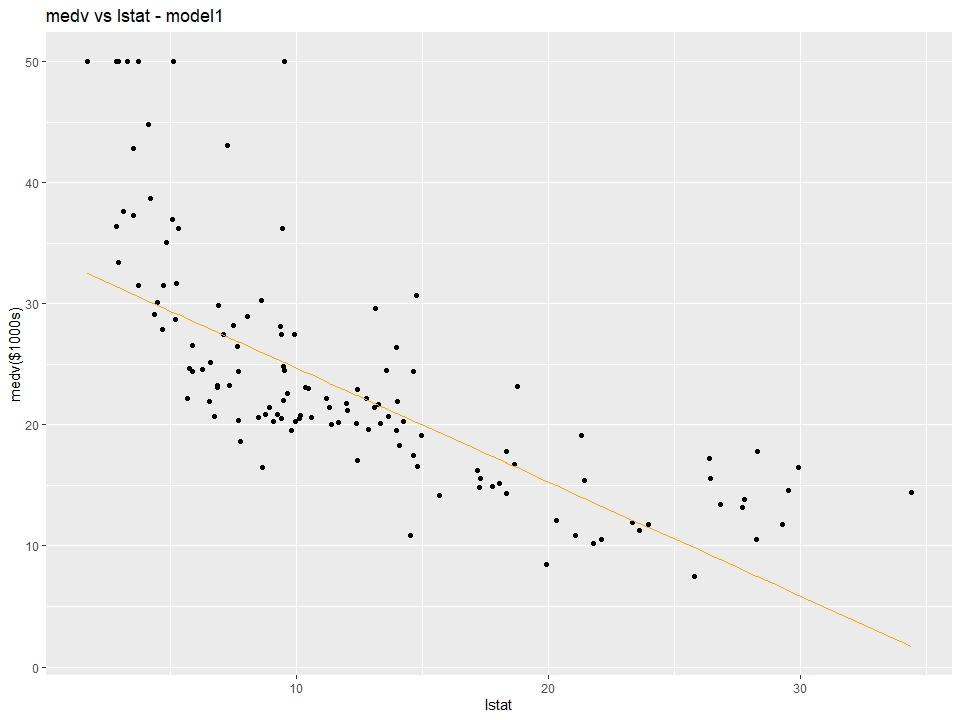
\includegraphics[width=0.7\linewidth]{model1}
	%\caption{基于Wolfe条件的线搜索算法}
	\label{bdc1}
\end{figure}

计算其在测试集上的均方根误差RMSE:
\begin{Shaded}
	\begin{Highlighting}[]
\NormalTok{model1.rmse<-}\KeywordTok{rmse}\NormalTok{(Boston.test[,}\DecValTok{14}\NormalTok{],model1.evaluate)}
\NormalTok{model1.rmse}
	\end{Highlighting}
\end{Shaded}

\begin{verbatim}
## [1] 6.83024
\end{verbatim}

查看其diagnosis plot:

\begin{Shaded}
	\begin{Highlighting}[]
\KeywordTok{plot}\NormalTok{(model.slm)}
	\end{Highlighting}
\end{Shaded}

\begin{figure}[H]
	\centering
	\subfigure[]{
		\begin{minipage}[t]{0.5\linewidth}
			\centering
			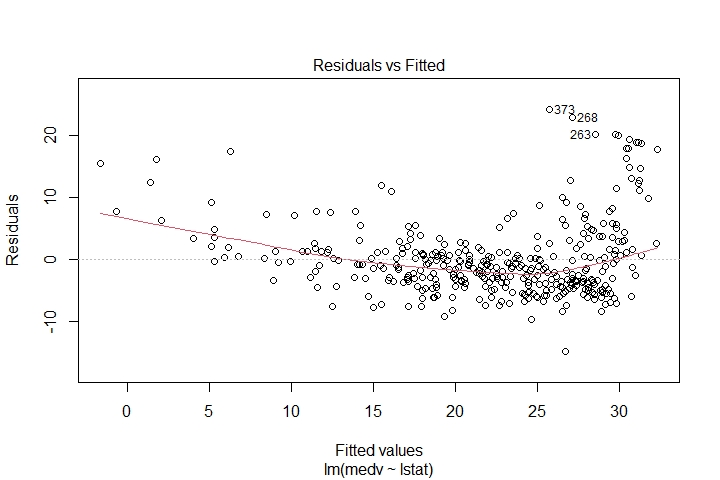
\includegraphics[width=3.5in]{1dp1}
			%\caption{fig1}
		\end{minipage}%
	}%
	\subfigure[]{
		\begin{minipage}[t]{0.5\linewidth}
			\centering
			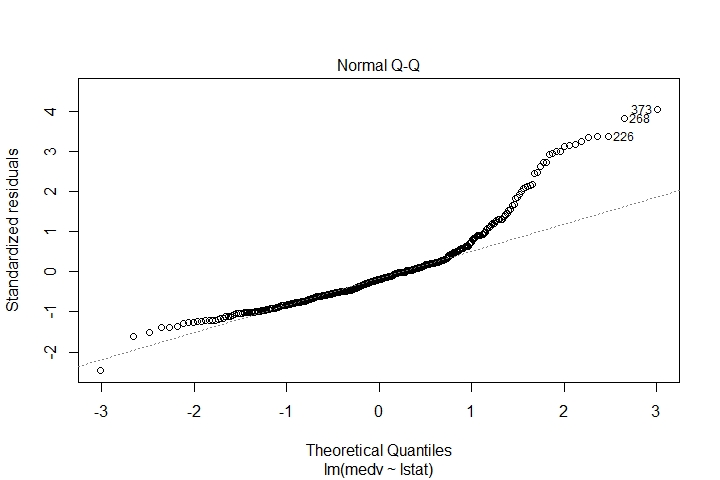
\includegraphics[width=3.5in]{1dp2}
			%\caption{fig2}
		\end{minipage}%
	}%
	\centering
\end{figure}H
%	\caption{处理效果的整体呈现}	
\begin{figure}[H]
	\centering
	\subfigure[]{
		\begin{minipage}[t]{0.5\linewidth}
			\centering
			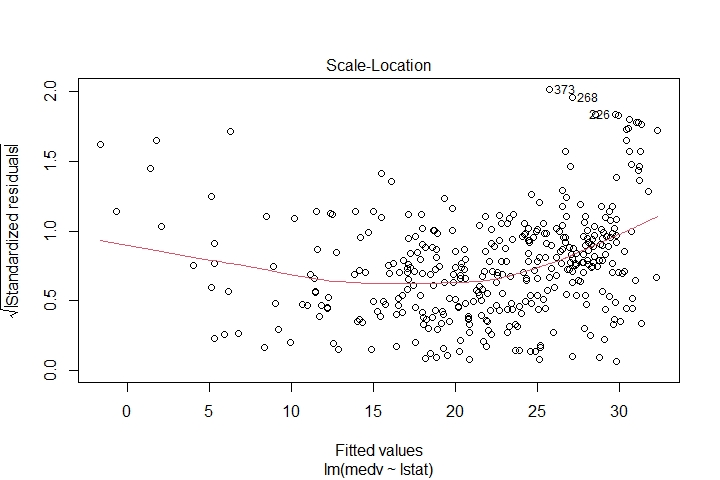
\includegraphics[width=3.5in]{1dp3}
			%\caption{fig2}
		\end{minipage}%
	}%
	\subfigure[]{
		\begin{minipage}[t]{0.5\linewidth}
			\centering
			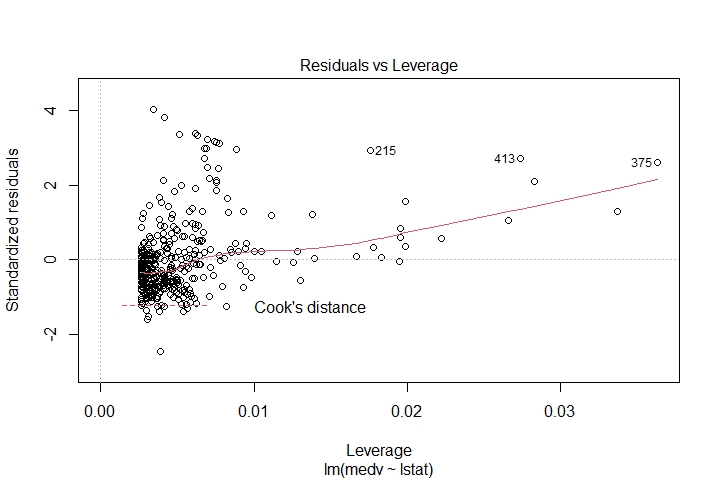
\includegraphics[width=3.5in]{1dp4}
			%\caption{fig2}
		\end{minipage}%
	}%
	\centering
	%	\caption{处理效果的整体呈现}
\end{figure}
第一张图表明在medv和lstat之间可能存在非线性项,因此我们考虑构造单变量非线性回归模型。


\subsection{4.2 单变量非线性回归模型}

在单变量线性回归模型medv\textasciitilde lstat的基础上,我们添加lstat的非线性项\(lstat^{2}\),即:

\begin{Shaded}
	\begin{Highlighting}[]
\NormalTok{model.snlm=}\KeywordTok{lm}\NormalTok{(medv}\OperatorTok{~}\NormalTok{lstat}\OperatorTok{+}\KeywordTok{I}\NormalTok{(lstat}\OperatorTok{^}\DecValTok{2}\NormalTok{),}\DataTypeTok{data=}\NormalTok{Boston.train)}
	\end{Highlighting}
\end{Shaded}

同样,查看其统计量:

\begin{Shaded}
	\begin{Highlighting}[]
\KeywordTok{summary}\NormalTok{(model.snlm)}
	\end{Highlighting}
\end{Shaded}

\begin{verbatim}
## 
## Call:
## lm(formula = medv ~ lstat + I(lstat^2), data = Boston.train)
## 
## Residuals:
##      Min       1Q   Median       3Q      Max 
## -15.0041  -3.8585  -0.6233   2.3328  24.6350 
## 
## Coefficients:
##              Estimate Std. Error t value Pr(>|t|)    
## (Intercept) 41.791558   0.988539  42.276   <2e-16 ***
## lstat       -2.199963   0.137861 -15.958   <2e-16 ***
## I(lstat^2)   0.039428   0.004141   9.522   <2e-16 ***
## ---
## Signif. codes:  0 '***' 0.001 '**' 0.01 '*' 0.05 '.' 0.1 ' ' 1
## 
## Residual standard error: 5.399 on 376 degrees of freedom
## Multiple R-squared:  0.6388, Adjusted R-squared:  0.6369 
## F-statistic: 332.5 on 2 and 376 DF,  p-value: < 2.2e-16
\end{verbatim}

结果显示T检验的截距和自变量lstat都是非常显著,且相比于线性模型,相关系数的\(R^{2}\)检验值也显著增加。接下来在测试集上进行预测:

\begin{Shaded}
	\begin{Highlighting}[]
\NormalTok{model2.evaluate<-}\KeywordTok{predict}\NormalTok{(model.snlm, Boston.test) }
\KeywordTok{ggplot}\NormalTok{(}\DataTypeTok{data =}\NormalTok{ Boston.test) }\OperatorTok{+}
\StringTok{  }\KeywordTok{geom_point}\NormalTok{(}\KeywordTok{aes}\NormalTok{(}\DataTypeTok{x =}\NormalTok{ lstat, }\DataTypeTok{y =}\NormalTok{ medv),}\DataTypeTok{col=}\StringTok{"black"}\NormalTok{) }\OperatorTok{+}
\StringTok{  }\KeywordTok{geom_line}\NormalTok{(}\KeywordTok{aes}\NormalTok{(}\DataTypeTok{x =}\NormalTok{ lstat, }\DataTypeTok{y =}\NormalTok{ model2.evaluate),}\DataTypeTok{col=}\StringTok{"orange"}\NormalTok{) }\OperatorTok{+}
\StringTok{  }\KeywordTok{labs}\NormalTok{(}\DataTypeTok{title =} \StringTok{"medv vs lstat - model2"}\NormalTok{,}
		\DataTypeTok{y =} \StringTok{"medv($1000s)"}\NormalTok{,}
		\DataTypeTok{x =} \StringTok{"lstat"}\NormalTok{)}
		\end{Highlighting}
		\end{Shaded}

\begin{figure}[H]
	\centering
	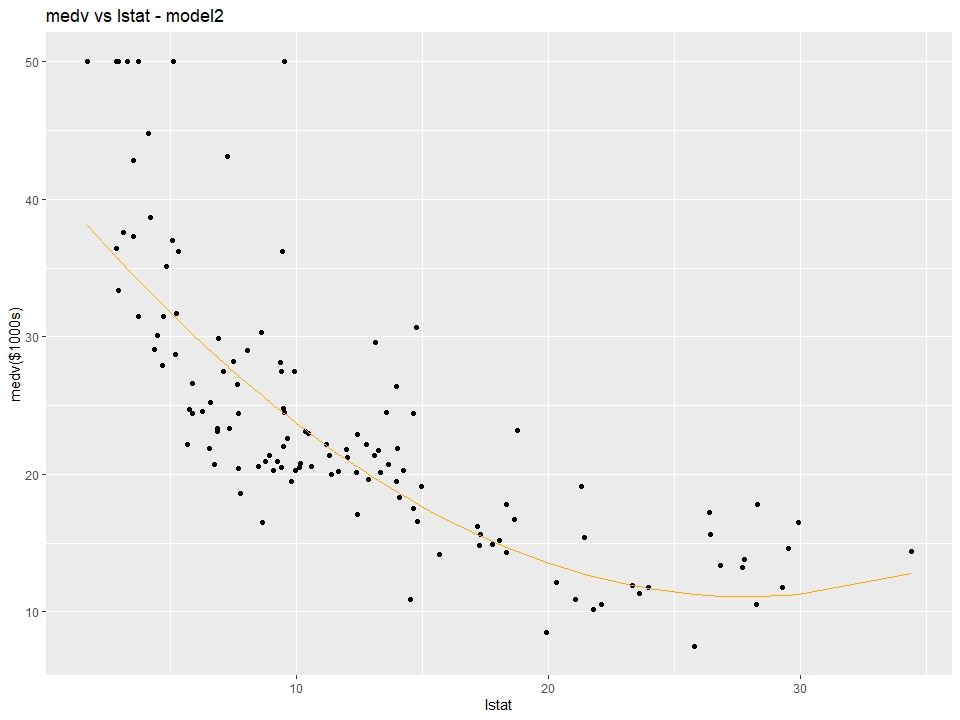
\includegraphics[width=0.7\linewidth]{model2}
	%\caption{基于Wolfe条件的线搜索算法}
	\label{bdc1}
\end{figure}

拟合效果明显优于简单的单变量线性模型。计算其在测试集上的RMSE:

\begin{Shaded}
	\begin{Highlighting}[]
\NormalTok{model2.rmse<-}\KeywordTok{rmse}\NormalTok{(Boston.test[,}\DecValTok{14}\NormalTok{],model2.evaluate)}
\NormalTok{model2.rmse}
	\end{Highlighting}
\end{Shaded}

\begin{verbatim}
## [1] 5.924323
\end{verbatim}

查看其Diagnostics plot:

\begin{Shaded}
	\begin{Highlighting}[]
\KeywordTok{plot}\NormalTok{(model.snlm)}
	\end{Highlighting}
\end{Shaded}

\begin{figure}[htbp]
	\centering
	\subfigure[]{
		\begin{minipage}[t]{0.5\linewidth}
			\centering
			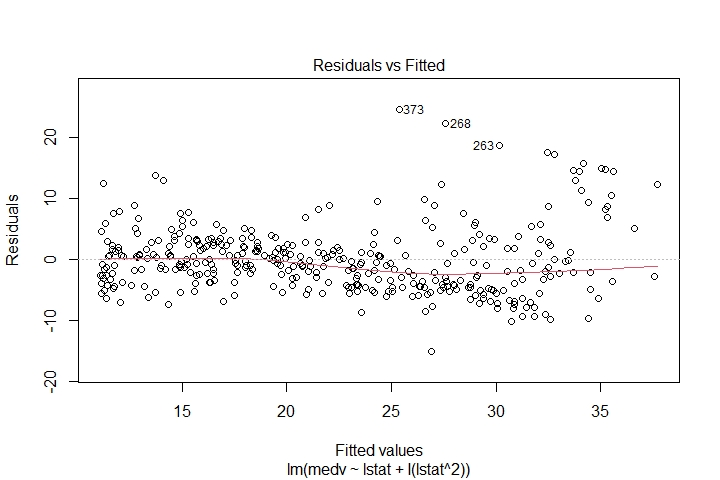
\includegraphics[width=3.5in]{2dp1}
			%\caption{fig1}
		\end{minipage}%
	}%
	\subfigure[]{
		\begin{minipage}[t]{0.5\linewidth}
			\centering
			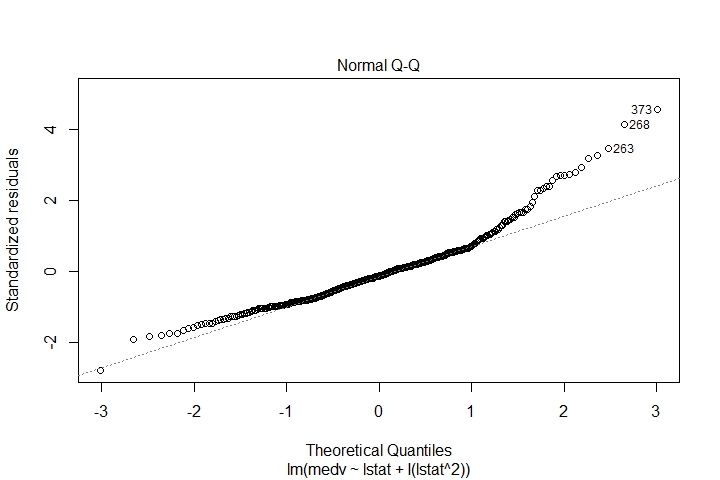
\includegraphics[width=3.5in]{2dp2}
			%\caption{fig2}
		\end{minipage}%
	}%
	
	\subfigure[]{
		\begin{minipage}[t]{0.5\linewidth}
			\centering
			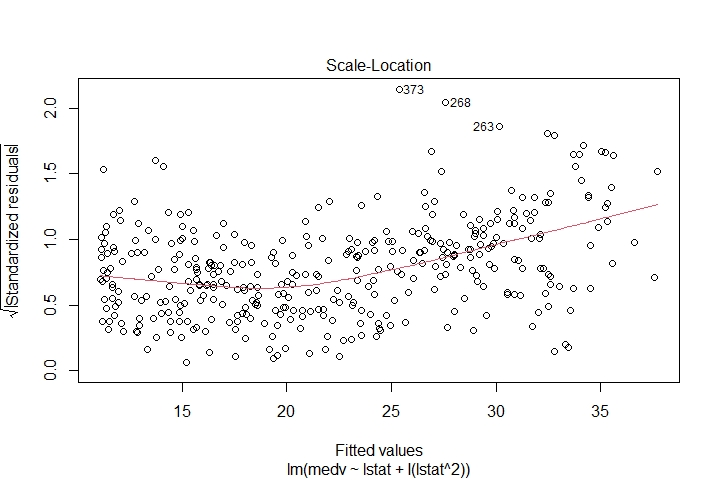
\includegraphics[width=3.5in]{2dp3}
			%\caption{fig2}
		\end{minipage}%
	}%
	\subfigure[]{
		\begin{minipage}[t]{0.5\linewidth}
			\centering
			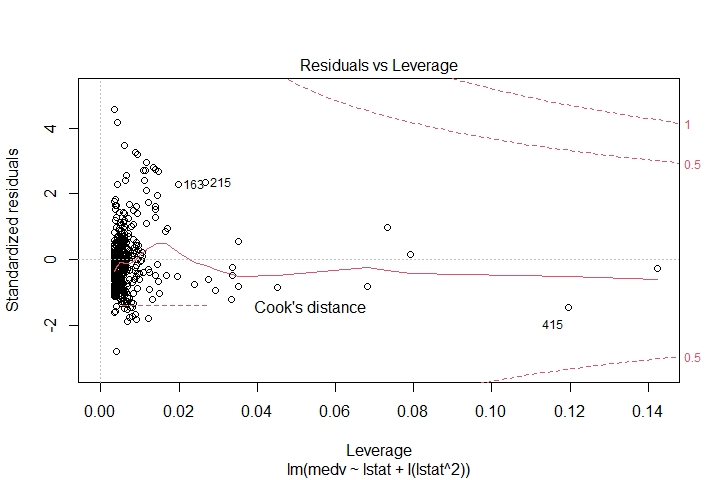
\includegraphics[width=3.5in]{2dp4}
			%\caption{fig2}
		\end{minipage}%
	}%
	\centering
	%	\caption{处理效果的整体呈现}
\end{figure}

通过添加非线性因子,我们将模型在测试集上预测的均方根误差有效降低,同时显著提高了对于模型的拟合效果。同时,上面图一显示模型需要进一步修改,我们考虑引入更多的变量来改进我们的模型。

\subsection{4.3 多变量回归模型}
通过引入更多的变量构造多变量回归模型,我们有两种思路:
\begin{itemize}
	\item 在上一节中拟合效果已经较好的的单变量非线性模型上添加变量
	\item 考虑使用广义加性模型Generalized
	Additive Models(GAM)
\end{itemize}

\subsubsection{4.3.1 单变量非线性回归模型基础上添加变量}
在不了解其经济社会学原理的情况下,将所有变量纳入考虑进行回归是最为稳妥的做法。即:

\begin{Shaded}
	\begin{Highlighting}[]
\NormalTok{model.mrm=}\KeywordTok{lm}\NormalTok{(medv}\OperatorTok{~}\NormalTok{crim}\OperatorTok{+}\NormalTok{zn}\OperatorTok{+}\NormalTok{indus}\OperatorTok{+}\NormalTok{chas}\OperatorTok{+}\NormalTok{nox}\OperatorTok{+}\NormalTok{rm}\OperatorTok{+}\NormalTok{age}\OperatorTok{+}\NormalTok{dis}\OperatorTok{+}\NormalTok{rad}\OperatorTok{+}\NormalTok{tax}\OperatorTok{+}
\StringTok{               }\NormalTok{ptratio}\OperatorTok{+}\NormalTok{black}\OperatorTok{+}\NormalTok{lstat}\OperatorTok{+}\KeywordTok{I}\NormalTok{(lstat}\OperatorTok{^}\DecValTok{2}\NormalTok{),}\DataTypeTok{data=}\NormalTok{Boston.train)}
	\end{Highlighting}
\end{Shaded}

查看其统计量:

\begin{Shaded}
	\begin{Highlighting}[]
\KeywordTok{summary}\NormalTok{(model.mrm)}
	\end{Highlighting}
\end{Shaded}

\begin{verbatim}
## 
## Call:
## lm(formula = medv ~ crim + zn + indus + chas + nox + rm + age + 
##     dis + rad + tax + ptratio + black + lstat + I(lstat^2), data = Boston.train)
## 
## Residuals:
##      Min       1Q   Median       3Q      Max 
## -15.5528  -2.3805  -0.3195   1.7342  24.7913 
## 
## Coefficients:
##               Estimate Std. Error t value Pr(>|t|)    
## (Intercept)  43.799421   5.151894   8.502 4.89e-16 ***
## crim         -0.135197   0.030422  -4.444 1.17e-05 ***
## zn            0.024778   0.014222   1.742 0.082318 .  
## indus         0.043005   0.060892   0.706 0.480485    
## chas          2.213046   0.889561   2.488 0.013301 *  
## nox         -19.393777   4.040227  -4.800 2.32e-06 ***
## rm            3.329732   0.448026   7.432 7.71e-13 ***
## age           0.021802   0.013471   1.618 0.106438    
## dis          -1.187884   0.214759  -5.531 6.08e-08 ***
## rad           0.334585   0.069606   4.807 2.25e-06 ***
## tax          -0.014200   0.003915  -3.627 0.000328 ***
## ptratio      -0.863652   0.130906  -6.598 1.48e-10 ***
## black         0.006460   0.002552   2.531 0.011787 *  
## lstat        -1.504056   0.143232 -10.501  < 2e-16 ***
## I(lstat^2)    0.029150   0.003678   7.925 2.82e-14 ***
## ---
## Signif. codes:  0 '***' 0.001 '**' 0.01 '*' 0.05 '.' 0.1 ' ' 1
## 
## Residual standard error: 4.156 on 364 degrees of freedom
## Multiple R-squared:  0.7928, Adjusted R-squared:  0.7848 
## F-statistic: 99.47 on 14 and 364 DF,  p-value: < 2.2e-16
\end{verbatim}

根据结果可以看出,zn,indus,chas,age和black这些变量的T检验是不显著的,其余的变量的T检验都是显著的。回归的整体\(R^{2}\)检验值相比较单变量非线性模型有所提高。

其次查看其在测试集上的表现:

\begin{Shaded}
	\begin{Highlighting}[]
\NormalTok{model3.evaluate<-}\KeywordTok{predict}\NormalTok{(model.mrm, Boston.test) }
\KeywordTok{ggplot}\NormalTok{(}\DataTypeTok{data =}\NormalTok{ Boston.test) }\OperatorTok{+}
\StringTok{  }\KeywordTok{geom_point}\NormalTok{(}\KeywordTok{aes}\NormalTok{(}\DataTypeTok{x =}\NormalTok{ lstat, }\DataTypeTok{y =}\NormalTok{ medv),}\DataTypeTok{col=}\StringTok{"black"}\NormalTok{) }\OperatorTok{+}
\StringTok{  }\KeywordTok{geom_line}\NormalTok{(}\KeywordTok{aes}\NormalTok{(}\DataTypeTok{x =}\NormalTok{ lstat, }\DataTypeTok{y =}\NormalTok{ model3.evaluate),}\DataTypeTok{col=}\StringTok{"orange"}\NormalTok{) }\OperatorTok{+}
\StringTok{  }\KeywordTok{labs}\NormalTok{(}\DataTypeTok{title =} \StringTok{"medv vs lstat - model3"}\NormalTok{,}
\DataTypeTok{y =} \StringTok{"medv($1000s)"}\NormalTok{,}
		\DataTypeTok{x =} \StringTok{"lstat"}\NormalTok{)}
		\end{Highlighting}
		\end{Shaded}

\begin{figure}[H]
	\centering
	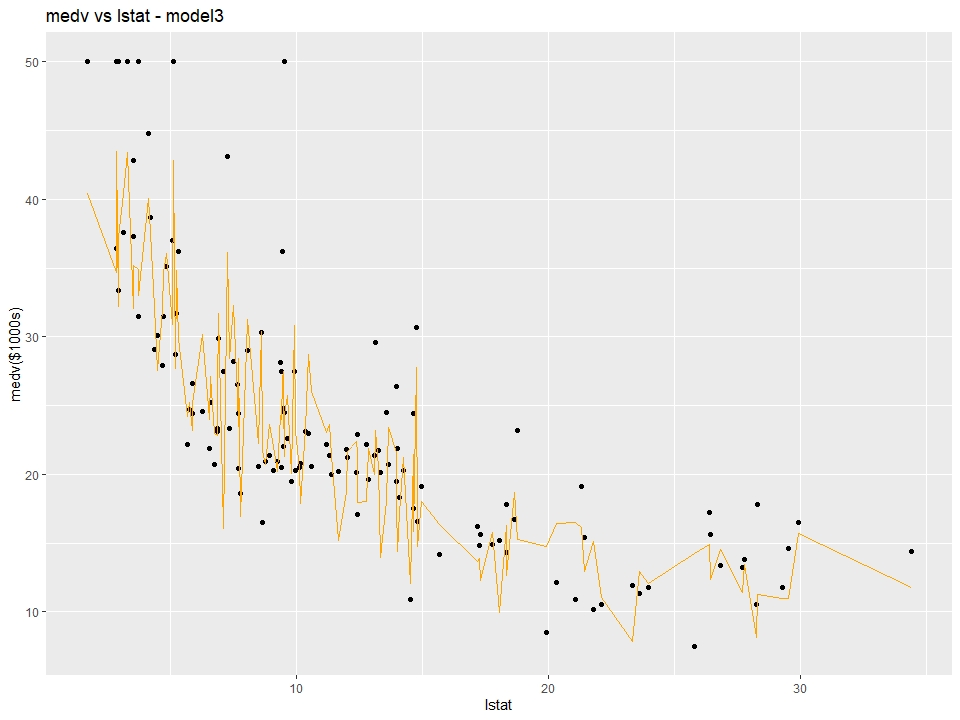
\includegraphics[width=0.7\linewidth]{model3}
	%\caption{基于Wolfe条件的线搜索算法}
	\label{bdc1}
\end{figure}		

计算其在测试集上的RMSE,相比之前有了进一步的下降:

\begin{Shaded}
	\begin{Highlighting}[]
\NormalTok{model3.rmse<-}\KeywordTok{rmse}\NormalTok{(Boston.test[,}\DecValTok{14}\NormalTok{],model3.evaluate)}
\NormalTok{model3.rmse}
	\end{Highlighting}
\end{Shaded}

\begin{verbatim}
## [1] 4.792194
\end{verbatim}

查看其Diagnostics plot:
\begin{Shaded}
	\begin{Highlighting}[]
\KeywordTok{plot}\NormalTok{(model.mrm)}
	\end{Highlighting}
\end{Shaded}

\begin{figure}[H]
	\centering
	\subfigure[]{
		\begin{minipage}[t]{0.5\linewidth}
			\centering
			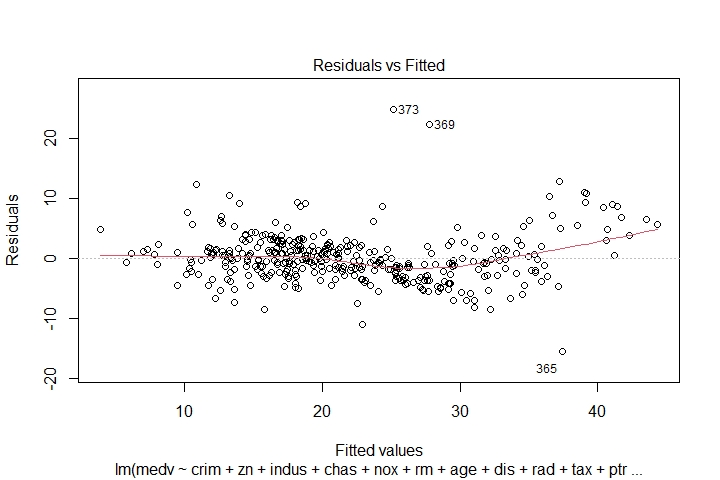
\includegraphics[width=3.5in]{3dp1}
			%\caption{fig1}
		\end{minipage}%
	}%
	\subfigure[]{
		\begin{minipage}[t]{0.5\linewidth}
			\centering
			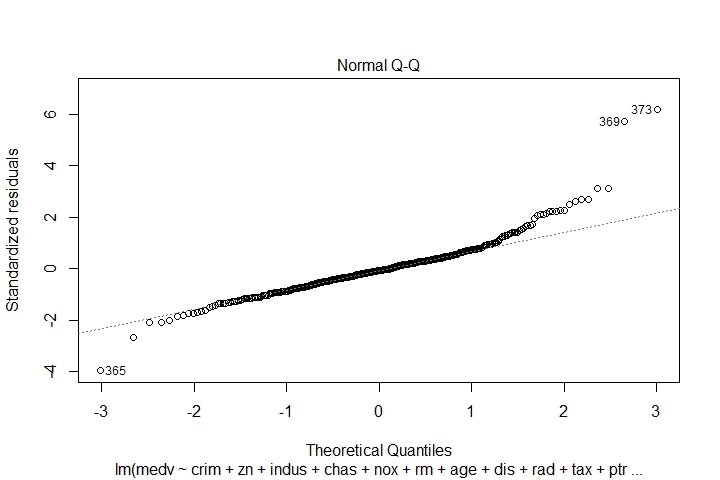
\includegraphics[width=3.5in]{3dp2}
			%\caption{fig2}
		\end{minipage}%
	}%
	
	\subfigure[]{
		\begin{minipage}[t]{0.5\linewidth}
			\centering
			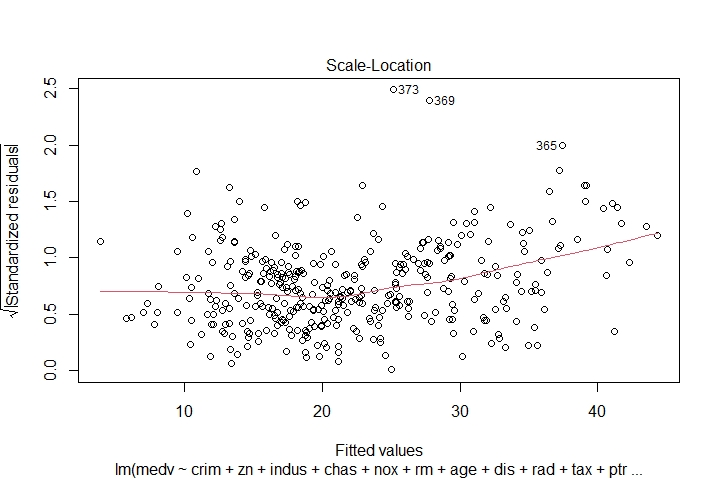
\includegraphics[width=3.5in]{3dp3}
			%\caption{fig2}
		\end{minipage}%
	}%
	\subfigure[]{
		\begin{minipage}[t]{0.5\linewidth}
			\centering
			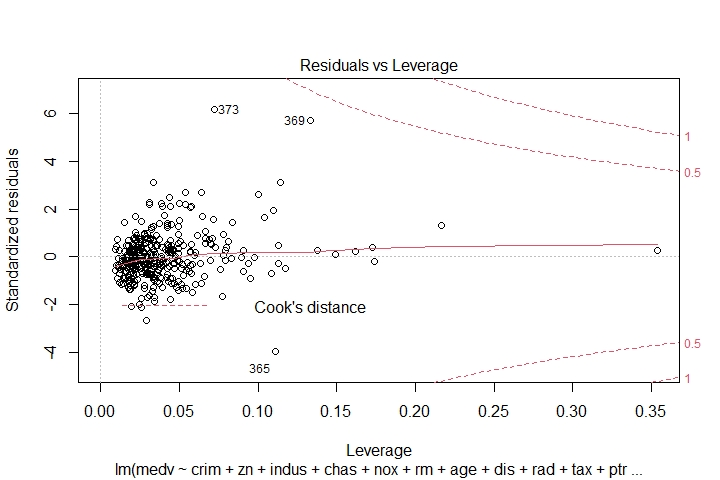
\includegraphics[width=3.5in]{3dp4}
			%\caption{fig2}
		\end{minipage}%
	}%
	\centering
	%	\caption{处理效果的整体呈现}
\end{figure}
图一显示,模型中某些变量和medv可能并不是线性关系,我们仍需要进一步改进模型,因而考虑引入广义加性模型。

\subsubsection{4.3.1 广义加性模型GAM}

在上面的多变量回归中,除lstat外,新引入的变量均以线性形式存在,然而实际情况并不一定如此,但我们并不清楚其具体的存在形式,因此我们考虑利用GAM,对部分变量使用光滑样条函数来拟合。

首先,变量chas和rad是不连续的,因此不适宜使用光滑样条函数拟合,除此之外的变量我们尝试均用样条函数拟合,建立模型:

\begin{Shaded}
	\begin{Highlighting}[]
\NormalTok{model.gam}\FloatTok{.0}\NormalTok{ <-}\StringTok{ }\KeywordTok{gam}\NormalTok{(medv }\OperatorTok{~}\StringTok{ }\KeywordTok{s}\NormalTok{(crim) }\OperatorTok{+}\StringTok{ }\KeywordTok{s}\NormalTok{(zn) }\OperatorTok{+}\StringTok{ }\KeywordTok{s}\NormalTok{(indus) }\OperatorTok{+}\StringTok{ }\KeywordTok{s}\NormalTok{(nox) }\OperatorTok{+}
\StringTok{                   }\KeywordTok{s}\NormalTok{(rm) }\OperatorTok{+}\StringTok{ }\KeywordTok{s}\NormalTok{(age) }\OperatorTok{+}\StringTok{ }\KeywordTok{s}\NormalTok{(dis) }\OperatorTok{+}\StringTok{ }
\StringTok{                   }\KeywordTok{s}\NormalTok{(tax) }\OperatorTok{+}\StringTok{ }\KeywordTok{s}\NormalTok{(ptratio) }\OperatorTok{+}\StringTok{ }\KeywordTok{s}\NormalTok{(black) }\OperatorTok{+}\StringTok{ }
\StringTok{                   }\KeywordTok{s}\NormalTok{(lstat) }\OperatorTok{+}\StringTok{ }\NormalTok{chas }\OperatorTok{+}\StringTok{ }\NormalTok{rad, }\DataTypeTok{data =}\NormalTok{ Boston.train)}
\KeywordTok{summary}\NormalTok{(model.gam}\FloatTok{.0}\NormalTok{)}
	\end{Highlighting}
\end{Shaded}

\begin{verbatim}
## 
## Family: gaussian 
## Link function: identity 
## 
## Formula:
## medv ~ s(crim) + s(zn) + s(indus) + s(nox) + s(rm) + s(age) + 
##     s(dis) + s(tax) + s(ptratio) + s(black) + s(lstat) + chas + 
##     rad
## 
## Parametric coefficients:
##             Estimate Std. Error t value Pr(>|t|)    
## (Intercept)  17.6497     1.0417  16.943  < 2e-16 ***
## chas          0.4137     0.7019   0.589    0.556    
## rad           0.4537     0.1054   4.304 2.22e-05 ***
## ---
## Signif. codes:  0 '***' 0.001 '**' 0.01 '*' 0.05 '.' 0.1 ' ' 1
## 
## Approximate significance of smooth terms:
##              edf Ref.df      F  p-value    
## s(crim)    3.073  3.838 10.275 1.85e-07 ***
## s(zn)      1.000  1.000  1.267    0.261    
## s(indus)   4.009  4.910  1.018    0.452    
## s(nox)     8.800  8.976 11.651 4.92e-16 ***
## s(rm)      8.119  8.763 27.424  < 2e-16 ***
## s(age)     1.000  1.000  0.145    0.704    
## s(dis)     8.679  8.963  5.737 2.23e-07 ***
## s(tax)     3.254  3.932  7.250 1.49e-05 ***
## s(ptratio) 1.000  1.000 38.074 1.87e-09 ***
## s(black)   1.497  1.832  1.766    0.261    
## s(lstat)   4.638  5.767 21.709  < 2e-16 ***
## ---
## Signif. codes:  0 '***' 0.001 '**' 0.01 '*' 0.05 '.' 0.1 ' ' 1
## 
## R-sq.(adj) =  0.888   Deviance explained = 90.2%
## GCV = 10.293  Scale est. = 8.9876    n = 379
\end{verbatim}

edf统计量接近1的变量可能和medv具有线性关系,因此再结合p检验值分析,上述结果中的zn,age,black以及ptratio同medv可能是线性关系,其他的变量仍用样条函数拟合,同时剔除indus,对模型调整如下:

\begin{Shaded}
	\begin{Highlighting}[]
\NormalTok{model.gam}\FloatTok{.1}\NormalTok{ <-}\StringTok{ }\KeywordTok{gam}\NormalTok{(medv }\OperatorTok{~}\StringTok{ }\KeywordTok{s}\NormalTok{(crim) }\OperatorTok{+}\StringTok{ }\NormalTok{zn  }\OperatorTok{+}\StringTok{ }\KeywordTok{s}\NormalTok{(nox) }\OperatorTok{+}
\StringTok{                   }\KeywordTok{s}\NormalTok{(rm) }\OperatorTok{+}\StringTok{ }\NormalTok{age }\OperatorTok{+}\StringTok{ }\KeywordTok{s}\NormalTok{(dis) }\OperatorTok{+}\StringTok{ }
\StringTok{                   }\KeywordTok{s}\NormalTok{(tax) }\OperatorTok{+}\StringTok{ }\NormalTok{ptratio }\OperatorTok{+}\StringTok{ }\NormalTok{black }\OperatorTok{+}\StringTok{ }
\StringTok{                   }\KeywordTok{s}\NormalTok{(lstat) }\OperatorTok{+}\StringTok{ }\NormalTok{chas }\OperatorTok{+}\StringTok{ }\NormalTok{rad, }\DataTypeTok{data =}\NormalTok{ Boston.train)}
\KeywordTok{summary}\NormalTok{(model.gam}\FloatTok{.1}\NormalTok{)}
	\end{Highlighting}
\end{Shaded}

\begin{verbatim}
## 
## Family: gaussian 
## Link function: identity 
## 
## Formula:
## medv ~ s(crim) + zn + s(nox) + s(rm) + age + s(dis) + s(tax) + 
##     ptratio + black + s(lstat) + chas + rad
## 
## Parametric coefficients:
##              Estimate Std. Error t value Pr(>|t|)    
## (Intercept) 30.485739   2.540361  12.001  < 2e-16 ***
## zn           0.012390   0.013494   0.918    0.359    
## age         -0.007073   0.011298  -0.626    0.532    
## ptratio     -0.717569   0.111394  -6.442 4.09e-10 ***
## black        0.002959   0.002097   1.411    0.159    
## chas         0.562623   0.686614   0.819    0.413    
## rad          0.426652   0.081793   5.216 3.20e-07 ***
## ---
## Signif. codes:  0 '***' 0.001 '**' 0.01 '*' 0.05 '.' 0.1 ' ' 1
## 
## Approximate significance of smooth terms:
##            edf Ref.df      F  p-value    
## s(crim)  3.088  3.869 10.484 8.29e-08 ***
## s(nox)   8.562  8.923 10.890 2.76e-15 ***
## s(rm)    8.006  8.722 28.486  < 2e-16 ***
## s(dis)   8.745  8.978  6.310 2.64e-08 ***
## s(tax)   3.073  3.716  7.371 2.31e-05 ***
## s(lstat) 4.682  5.819 21.655  < 2e-16 ***
## ---
## Signif. codes:  0 '***' 0.001 '**' 0.01 '*' 0.05 '.' 0.1 ' ' 1
## 
## R-sq.(adj) =  0.886   Deviance explained = 89.9%
## GCV = 10.283  Scale est. = 9.1122    n = 379
\end{verbatim}

进一步,剔除显著性极低的zn,age,black和chas变量,调整模型为:

\begin{Shaded}
	\begin{Highlighting}[]
\NormalTok{model.gam <-}\StringTok{ }\KeywordTok{gam}\NormalTok{(medv }\OperatorTok{~}\StringTok{ }\KeywordTok{s}\NormalTok{(crim)  }\OperatorTok{+}\StringTok{ }\KeywordTok{s}\NormalTok{(nox) }\OperatorTok{+}\KeywordTok{s}\NormalTok{(rm) }\OperatorTok{+}\StringTok{ }\KeywordTok{s}\NormalTok{(dis) }\OperatorTok{+}\StringTok{ }
\StringTok{            }\KeywordTok{s}\NormalTok{(tax) }\OperatorTok{+}\StringTok{ }\NormalTok{ptratio }\OperatorTok{+}\StringTok{ }\KeywordTok{s}\NormalTok{(lstat)  }\OperatorTok{+}\StringTok{ }\NormalTok{rad, }
\DataTypeTok{data =}\NormalTok{ Boston.train)}
\KeywordTok{summary}\NormalTok{(model.gam)}
	\end{Highlighting}
\end{Shaded}

\begin{verbatim}
## 
## Family: gaussian 
## Link function: identity 
## 
## Formula:
## medv ~ s(crim) + s(nox) + s(rm) + s(dis) + s(tax) + ptratio + 
##     s(lstat) + rad
## 
## Parametric coefficients:
##             Estimate Std. Error t value Pr(>|t|)    
## (Intercept) 31.65564    2.20861  14.333  < 2e-16 ***
## ptratio     -0.74255    0.10864  -6.835 3.81e-11 ***
## rad          0.42896    0.08124   5.280 2.31e-07 ***
## ---
## Signif. codes:  0 '***' 0.001 '**' 0.01 '*' 0.05 '.' 0.1 ' ' 1
## 
## Approximate significance of smooth terms:
##            edf Ref.df      F  p-value    
## s(crim)  3.079  3.857 12.125 5.61e-09 ***
## s(nox)   8.545  8.917 11.329 8.03e-16 ***
## s(rm)    8.005  8.722 29.441  < 2e-16 ***
## s(dis)   8.766  8.981  7.375 6.67e-10 ***
## s(tax)   3.137  3.794  7.447 1.59e-05 ***
## s(lstat) 4.796  5.936 28.008  < 2e-16 ***
## ---
## Signif. codes:  0 '***' 0.001 '**' 0.01 '*' 0.05 '.' 0.1 ' ' 1
## 
## R-sq.(adj) =  0.887   Deviance explained = 89.8%
## GCV = 10.141  Scale est. = 9.0884    n = 379
\end{verbatim}

可见各变量的显著程度明显增大,且\(R^{2}\)检验值相比之前显著提高,拟合程度优良,且各变量的显著性都很高,得到了较好的统计性质。

GAM模型中个变量和medv的非线性关系如下图所示:

\begin{Shaded}
	\begin{Highlighting}[]
\KeywordTok{plot}\NormalTok{(model.gam, }\DataTypeTok{shade =} \OtherTok{TRUE}\NormalTok{, }\DataTypeTok{seWithMean =} \OtherTok{TRUE}\NormalTok{, }\DataTypeTok{scale =} \DecValTok{0}\NormalTok{)}
	\end{Highlighting}
\end{Shaded}H

\begin{figure}[H]
	\centering
	\subfigure[]{
		\begin{minipage}[t]{0.5\linewidth}
			\centering
			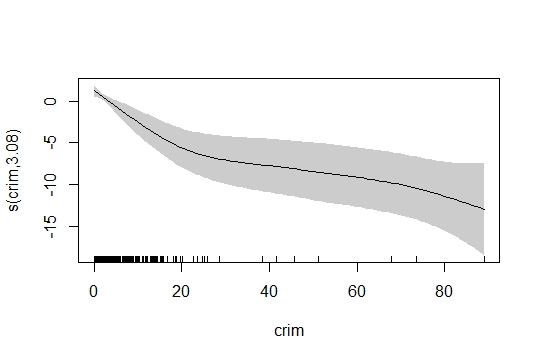
\includegraphics[width=3.5in]{4g1}
			%\caption{fig1}
		\end{minipage}%
	}%
	\subfigure[]{
		\begin{minipage}[t]{0.5\linewidth}
			\centering
			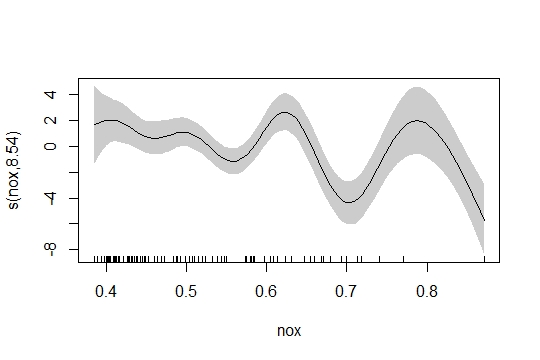
\includegraphics[width=3.5in]{4g2}
			%\caption{fig2}
		\end{minipage}%
	}%
	
	
	\subfigure[]{
		\begin{minipage}[t]{0.5\linewidth}
			\centering
			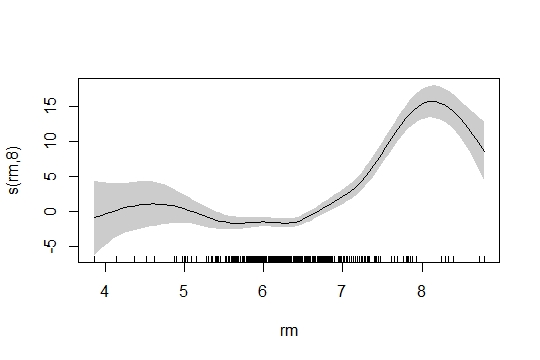
\includegraphics[width=3.5in]{4g3}
			%\caption{fig2}
		\end{minipage}%
	}%
	\subfigure[]{
		\begin{minipage}[t]{0.5\linewidth}
			\centering
			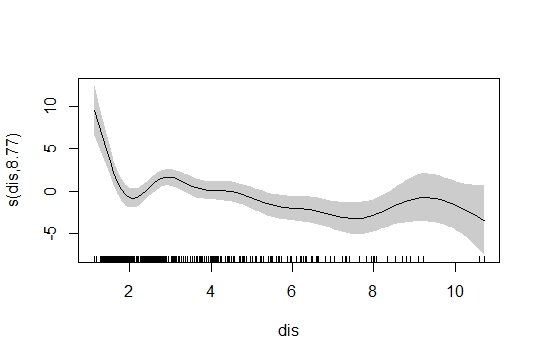
\includegraphics[width=3.5in]{4g4}
			%\caption{fig2}
		\end{minipage}%
	}%
	
	\subfigure[]{
		\begin{minipage}[t]{0.5\linewidth}
			\centering
			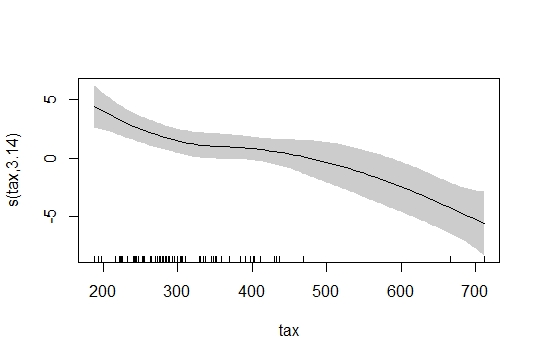
\includegraphics[width=3.5in]{4g5}
			%\caption{fig2}
		\end{minipage}%
	}%
	\subfigure[]{
		\begin{minipage}[t]{0.5\linewidth}
			\centering
			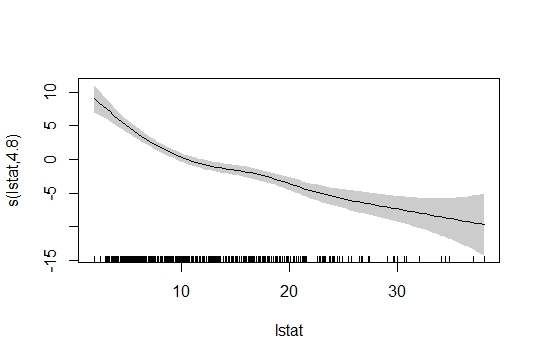
\includegraphics[width=3.5in]{4g6}
			%\caption{fig2}
		\end{minipage}%
	}%
	\centering
	%	\caption{处理效果的整体呈现}
\end{figure}

观察GAM模型在测试集上的表现:

\begin{Shaded}
	\begin{Highlighting}[]
\NormalTok{model4.evaluate<-}\KeywordTok{predict}\NormalTok{(model.gam, Boston.test) }
\KeywordTok{ggplot}\NormalTok{(}\DataTypeTok{data =}\NormalTok{ Boston.test) }\OperatorTok{+}
\StringTok{  }\KeywordTok{geom_point}\NormalTok{(}\KeywordTok{aes}\NormalTok{(}\DataTypeTok{x =}\NormalTok{ lstat, }\DataTypeTok{y =}\NormalTok{ medv),}\DataTypeTok{col=}\StringTok{"black"}\NormalTok{) }\OperatorTok{+}
\StringTok{  }\KeywordTok{geom_line}\NormalTok{(}\KeywordTok{aes}\NormalTok{(}\DataTypeTok{x =}\NormalTok{ lstat, }\DataTypeTok{y =}\NormalTok{ model4.evaluate),}\DataTypeTok{col=}\StringTok{"orange"}\NormalTok{) }\OperatorTok{+}
\StringTok{  }\KeywordTok{labs}\NormalTok{(}\DataTypeTok{title =} \StringTok{"medv vs lstat - model4"}\NormalTok{,}
		\DataTypeTok{y =} \StringTok{"medv($1000s)"}\NormalTok{,}
		\DataTypeTok{x =} \StringTok{"lstat"}\NormalTok{)}
		\end{Highlighting}
		\end{Shaded}

\begin{figure}[H]
	\centering
	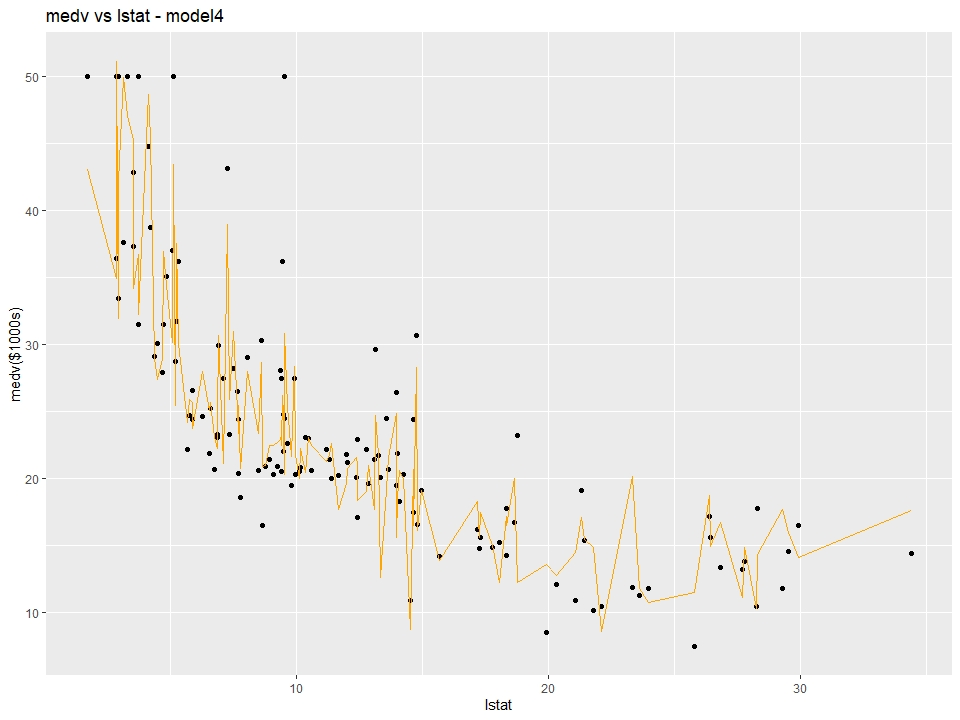
\includegraphics[width=0.7\linewidth]{model4}
	%\caption{基于Wolfe条件的线搜索算法}
	\label{bdc1}
\end{figure}

计算其在测试集上的RMSE,相比之前的模型有显著降低:
		
		\begin{Shaded}
			\begin{Highlighting}[]
\NormalTok{model4.rmse<-}\KeywordTok{rmse}\NormalTok{(Boston.test[,}\DecValTok{14}\NormalTok{],model4.evaluate)}
\NormalTok{model4.rmse}
			\end{Highlighting}
		\end{Shaded}
	
\begin{verbatim}
## [1] 4.056175
\end{verbatim}

\section{5 总结分析}

1、综合上述分析,以medv指标衡量的波士顿郊区房屋价格水平受多方面因素影响,其中crim、nox、rm、dis、tax和lstat等因素的影响作用最为显著.

2、以在测试集上的RMSE为主要评价指标,综合统计量和统计检验对比,上述四种模型中,GAM模型在测试集合上的表现最为优秀,即拟合和预测效果最好,可以较为客观科学地对房价水平进行评估预测.

3、在构建多变量回归模型过程中,我选择提出了统计检验中不显著的变量,这并非一种严谨的方式,因为在不了解其社会学原理和经济模型的前提下,贸然剔除任何因子都不稳妥.

4、多变量回归还有更多的方法,比如逐步回归,对变量选择和参数拟合也有更多的方法完成,受统计学知识所限,仍有改进空间。

\section{参考文献}

[1] Wickham, Hadley, Grolemund, Garrett. R for data science : import, tidy, transform, visualize, and model data[M]// R for Data Science: Import, Tidy, Transform, Visualize, and Model Data. O'Reilly Media, Inc. 2016.

[2] Maria L. Rizzo. Statistical Computing with R, Second Edtion[J]. Crc Press, 2016.

\end{document}

%%% Local Variables: 
%%% mode: latex
%%% TeX-master: t
%%% End: 
